\documentclass{article}
\usepackage{xcolor} % Add this line in the preamble

\usepackage{amsmath}
\usepackage{graphicx}
\usepackage[letterpaper, margin=0.5in]{geometry}
\usepackage{listings}
\usepackage{xcolor}

% MATLAB code formatting
\lstset{language=Matlab,
        basicstyle=\ttfamily\small,
        keywordstyle=\color{blue},
        commentstyle=\color{gray},
        stringstyle=\color{red},
        breaklines=true,
        frame=single,
        showstringspaces=false,
        numbers=left,
        numberstyle=\tiny\color{gray},
        stepnumber=1}
        
\title{EMCH 367 Controls - Homework 3}
\author{J. C. Vaught}
\date{Fall 2024}

\begin{document}

\maketitle

\section*{Problem 1 (60pt)}

Consider the following inverted pendulum system. The equation of motion is given by:

\begin{equation*}
(M + m) \ddot{x}(t) + b \dot{x}(t) = f(t) - ml \sin \theta(t) \dot{\theta}^2(t) + ml \cos \theta(t) \ddot{\theta}(t), \tag{1}
\end{equation*}
\begin{equation*}
(J + ml^2)\ddot{\theta}(t) - mgl \sin \theta(t) = ml \ddot{x}(t) \cos \theta(t). \tag{2}
\end{equation*}
\noindent
where \( M \) is the mass of the cart, \( m \) is the mass of the rod, \( l \) is the half-length of the rod, \( \theta \) is the angle of the rod with respect to the upright position, \( b \) is the coefficient of friction for the cart, and \( J \) is the moment of inertia of the rod. Assume that friction force is modeled as \( b\dot{x}(t) \).

\subsection*{(a) (10pt)}

Assume that we have small \( \theta \), that is, \( \theta \ll 1 \). Using the following simplifications:
\[
\sin \theta(t) \approx \theta(t), \quad \cos \theta(t) \approx 1, \quad \dot{\theta}^2(t) \approx 0,
\]
we can re-write the equations of motion as follows:

\begin{equation*}
\textcolor{blue}{(M + m) \ddot{x}(t) + b \dot{x}(t) = f(t) + ml \ddot{\theta}(t)}, \tag{1}
\end{equation*}
\begin{equation*}
\textcolor{blue}{(J + ml^2)\ddot{\theta}(t) = ml \ddot{x}(t) + mgl \theta(t)}. \tag{2}
\end{equation*}
\noindent
The key simplifications here are the approximations for small \( \theta \), where \( \sin \theta(t) \approx \theta(t) \) and \( \cos \theta(t) \approx 1 \). As a result, terms involving \( \dot{\theta}^2(t) \) vanish, and the equations become linear in \( \theta(t) \).


\newpage
\subsection*{(b) (10pt)}
Let \( M = 1 \, \text{kg}, \, m = 0.5 \, \text{kg}, \, b = 0.2 \, \text{N} \cdot \text{m}^{-1} \cdot \text{s}, \, l = 0.4 \, \text{m}, \, J = 0.01 \, \text{kg} \cdot \text{m}^2 \). Find the transfer function between \( \Theta(s) \) as an output and \( F(s) \) as an input, i.e., find \( \frac{\Theta(s)}{F(s)} \). Assume zero initial condition.


Given the system parameters:
\[
M = 1 \, \text{kg}, \quad m = 0.5 \, \text{kg}, \quad b = 0.2 \, \text{N/(m/s)}, \quad l = 0.4 \, \text{m}, \quad J = 0.01 \, \text{kg} \cdot \text{m}^2,
\]
and assuming zero initial conditions, we start with the linearized equations from part (a):

\begin{equation*}
(M + m) \ddot{x}(t) + b \dot{x}(t) = f(t) + ml \ddot{\theta}(t), \tag{1}
\end{equation*}
\begin{equation*}
(J + ml^2)\ddot{\theta}(t) = ml \ddot{x}(t) + mgl \theta(t). \tag{2}
\end{equation*}

Taking the Laplace transform of both equations (assuming zero initial conditions):

\[
(M + m) s^2 X(s) + b s X(s) = F(s) + ml s^2 \Theta(s), \tag{3}
\]
\[
(J + ml^2) s^2 \Theta(s) = ml s^2 X(s) + mgl \Theta(s). \tag{4}
\]

Solve Equation (3) for \( X(s) \):

\[
\left[ (M + m) s^2 + b s \right] X(s) = F(s) + ml s^2 \Theta(s),
\]
\[
X(s) = \frac{F(s) + ml s^2 \Theta(s)}{(M + m) s^2 + b s}. \tag{5}
\]

Substitute \( X(s) \) from Equation (5) into Equation (4):

\[
(J + ml^2) s^2 \Theta(s) = ml s^2 \left( \frac{F(s) + ml s^2 \Theta(s)}{(M + m) s^2 + b s} \right) + mgl \Theta(s) \tag{6}
\]

Multiply both sides by \( (M + m) s^2 + b s \):

\[
\left( J + ml^2 \right) s^2 \left( (M + m) s^2 + b s \right) \Theta(s) = ml s^2 \left[ F(s) + ml s^2 \Theta(s) \right] + mgl \left( (M + m) s^2 + b s \right) \Theta(s) \tag{7}
\]

Bring all terms involving \( \Theta(s) \) to one side:

\[
\left[(J + ml^2)[s^2]((M+m)[s^2]+bs) -mgl((M+m)(s^2)+bs)-(mls^2)(mls^2) \right] \Theta(s) = ml s^2 F(s) \tag{8}
\]

Simplify the left side:

\[
\left[(J + ml^2)(M+m)[s^4]+b(J + ml^2)[s^3] -mgl(M+m)[s^2]-mglb[s^1]-(ml)^2[s^4] \right] \Theta(s) = ml s^2 F(s) \tag{9}
\]

Combine all like terms
\[
\left[((J + ml^2)(M+m)-(ml)^2)[s^4]+b(J + ml^2)[s^3] -mgl(M+m)[s^2]-mglb[s^1] \right] \Theta(s) = ml s^2 F(s) \tag{10}
\]

Solve for \( \dfrac{\Theta(s)}{F(s)} \):

\[
\frac{\Theta(s)}{F(s)} = \frac{ml s^2}{\left( (J + ml^2)(M + m) - (ml)^2 \right) s^4 + (J + ml^2) b s^3 - mgl (M + m) s^2 - mgl b s} \tag{11}
\]

Next, substitute the given values for the parameters:
\[
M = 1 \, \text{kg}, \quad m = 0.5 \, \text{kg}, \quad b = 0.2 \, \text{N} \cdot \text{m}^{-1} \cdot \text{s}, \quad l = 0.4 \, \text{m}, \quad J = 0.01 \, \text{kg} \cdot \text{m}^2, \quad g = 9.8 \, \text{m/s}^2.
\]s

Substituting these numerical values into the equation:

\[
\left[ 0.095 s^4 + 0.018 s^3 - 2.94 s^2 - 0.392 s \right] \Theta(s) = 0.2 s^2 F(s).
\]

Finally, solve for the transfer function \( \frac{\Theta(s)}{F(s)} \):

\[
\boxed{\frac{\Theta(s)}{F(s)} = \frac{0.2 s^2}{0.095 s^4 + 0.018 s^3 - 2.94 s^2 - 0.392 s}}.
\]
\[
\boxed{\frac{\Theta(s)}{F(s)} = \frac{0.2 s}{0.095 s^3 + 0.018 s^2 - 2.94 s - 0.392}}.
\]
\newpage

\subsection*{(c) (10pt)}

Find the transfer function between \( X(s) \) as an output and \( F(s) \) as an input, i.e., find \( \dfrac{X(s)}{F(s)} \). Assume zero initial condition.

\textbf{Objective:} Find the transfer function \( \dfrac{X(s)}{F(s)} \).


\textbf{Starting with the linearized equations from part (a):}
\begin{equation*}
(M + m) \ddot{x}(t) + b \dot{x}(t) = f(t) + ml \ddot{\theta}(t), \tag{1}
\end{equation*}
\begin{equation*}
(J + ml^2)\ddot{\theta}(t) = ml \ddot{x}(t) + mgl \theta(t). \tag{2}
\end{equation*}


Taking the Laplace transform of both equations (zero initial conditions):

\[
(M + m) s^2 X(s) + b s X(s) = F(s) + ml s^2 \Theta(s), \tag{3}
\]
\[
(J + ml^2) s^2 \Theta(s) = ml s^2 X(s) + mgl \Theta(s). \tag{4}
\]

Solve Equation (4) for \( \Theta(s) \) in terms of \( X(s) \):

\[
\left[ (J + ml^2) s^2 - mgl \right] \Theta(s) = ml s^2 X(s),
\]
\[
\Theta(s) = \frac{ml s^2 X(s)}{\left( J + ml^2 \right) s^2 - mgl}. \tag{5}
\]

Substitute \( \Theta(s) \) into Equation (3):

\[
(M + m) s^2 X(s) + b s X(s) = F(s) + ml s^2 \left( \frac{ml s^2 X(s)}{\left( J + ml^2 \right) s^2 - mgl} \right).
\]

Simplify the right side:

\[
F(s) + \frac{(ml)^2 s^4 X(s)}{\left( J + ml^2 \right) s^2 - mgl}.
\]

Combine terms and solve for \( \dfrac{X(s)}{F(s)} \):

\[
\left[ (M + m) s^2 + b s - \frac{(ml)^2 s^4}{(J + ml^2) s^2 - mgl} \right] X(s) = F(s).
\]

Multiply both sides by \( D(s) = (J + ml^2) s^2 - mgl \):

\[
\left[ \left( M + m \right) s^2 + b s \right] ((J + ml^2) s^2 - mgl) X(s) - (ml)^2 s^4 X(s) = ((J + ml^2) s^2 - mgl) F(s).
\]

Solve for \( \dfrac{X(s)}{F(s)} \):

\[
\left\{ \left[ \left( M + m \right) s^2 + b s \right] ((J + ml^2) s^2 - mgl) - (ml)^2 s^4 \right\} X(s) = ((J + ml^2) s^2 - mgl) F(s).
\]

Thus, the transfer function is:

\[
\frac{X(s)}{F(s)} = \frac{((J + ml^2) s^2 - mgl)}{((M + m)s^2 + bs)((J + ml^2) s^2 - mgl) - (ml)^2 s^4}.
\]

Next, substitute the given values for the parameters:
\[
M = 1 \, \text{kg}, \quad m = 0.5 \, \text{kg}, \quad b = 0.2 \, \text{N} \cdot \text{m}^{-1} \cdot \text{s}, \quad l = 0.4 \, \text{m}, \quad J = 0.01 \, \text{kg} \cdot \text{m}^2, \quad g = 9.8 \, \text{m/s}^2.
\]

Substituting these numerical values into the equation:


\[
\boxed{\frac{X(s)}{F(s)} = \frac{0.09 s^2 - 1.96}{0.095 s^4 + 0.018 s^3 - 2.94 s^2 - 0.392 s}}
\]

\newpage

\subsection*{(d) (10pt)}

Using MATLAB, plot the impulse response of the transfer functions found in (b) and (c) for 1 second.

\begin{lstlisting}
clc
clear
close all
M = 1;          % Mass M in kg
m = 0.5;        % Mass m in kg
b = 0.2;        % Damping coefficient in N*m^{-1}*s
l = 0.4;        % Length l in meters
J = 0.01;       % Moment of inertia J in kg*m^2
g = 9.81;        % Acceleration due to gravity in m/s^2

% Calculations
ml = m * l;
ml2 = m * l^2;
ml_squared = (m * l)^2;
J_plus_ml2 = J + ml2;
M_plus_m = M + m;

%% Theta(s)/F(s)

% Denominator coefficients for Theta(s)/F(s)
a4 = (J_plus_ml2) * M_plus_m - ml_squared;  % s^4
a3 = (J_plus_ml2) * b;                      % s^3
a2 = -m * g * l * M_plus_m;                 % s^2
a1 = -m * g * l * b;                        % s^1
a0 = 0;                                     % s^0

den_theta = [a4, a3, a2, a1, a0];

% Numerator coefficients for Theta(s)/F(s)
num_theta = [0, 0, ml, 0, 0];

% Create the transfer function for Theta(s)/F(s)
sys_theta = tf(num_theta, den_theta);

% Time vector for 1 second
t = 0:0.01:1;  % Time from 0 to 1 second with step size 0.01

% Plot the impulse response for Theta(s)/F(s) for 1 second
figure;
impulse(sys_theta, t);
title('Impulse Response of \Theta(s)/F(s)');
xlabel('Time');
ylabel('\Theta (radians)');
grid on;

%% X(s)/F(s)

% Numerator coefficients for X(s)/F(s)
num_x = [J_plus_ml2, 0, -m * g * l];

% Denominator part 1: (M + m)s^2 + b s
den_part1 = [M_plus_m, b, 0];

% Denominator part 2: (J + ml^2)s^2 - mgl
den_part2 = [J_plus_ml2, 0, -m * g * l];

% Multiply den_part1 and den_part2
den_temp = conv(den_part1, den_part2);

% Subtract (ml)^2 s^4 term
ml_squared_s4 = [ml_squared, 0, 0, 0, 0];

% Ensure both arrays are the same length
len_diff = length(den_temp) - length(ml_squared_s4);
ml_squared_s4_padded = [ml_squared_s4, zeros(1, len_diff)];

% Final denominator coefficients for X(s)/F(s)
den_x = den_temp - ml_squared_s4_padded;

% Create the transfer function for X(s)/F(s)
sys_x = tf(num_x, den_x);

% Plot the impulse response for X(s)/F(s) for 1 second
figure;
impulse(sys_x, t);
title('Impulse Response of X(s)/F(s)');
xlabel('Time');
ylabel('X (meters)');
grid on;

\end{lstlisting}


\begin{figure}[h!]
    \centering
    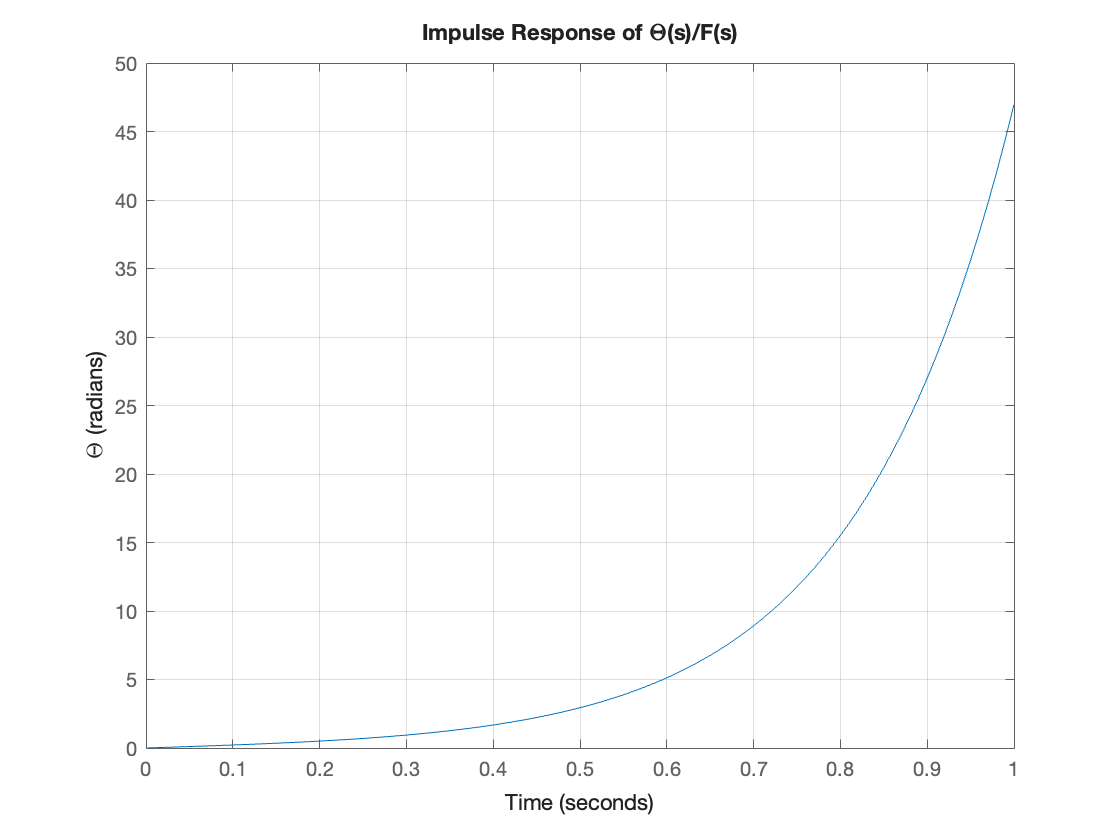
\includegraphics[width=0.5\textwidth]{p1db.png}
    \caption{Impulse Response of $\Theta$(s)/F(s)}
\end{figure}

\begin{figure}[h!]
    \centering
    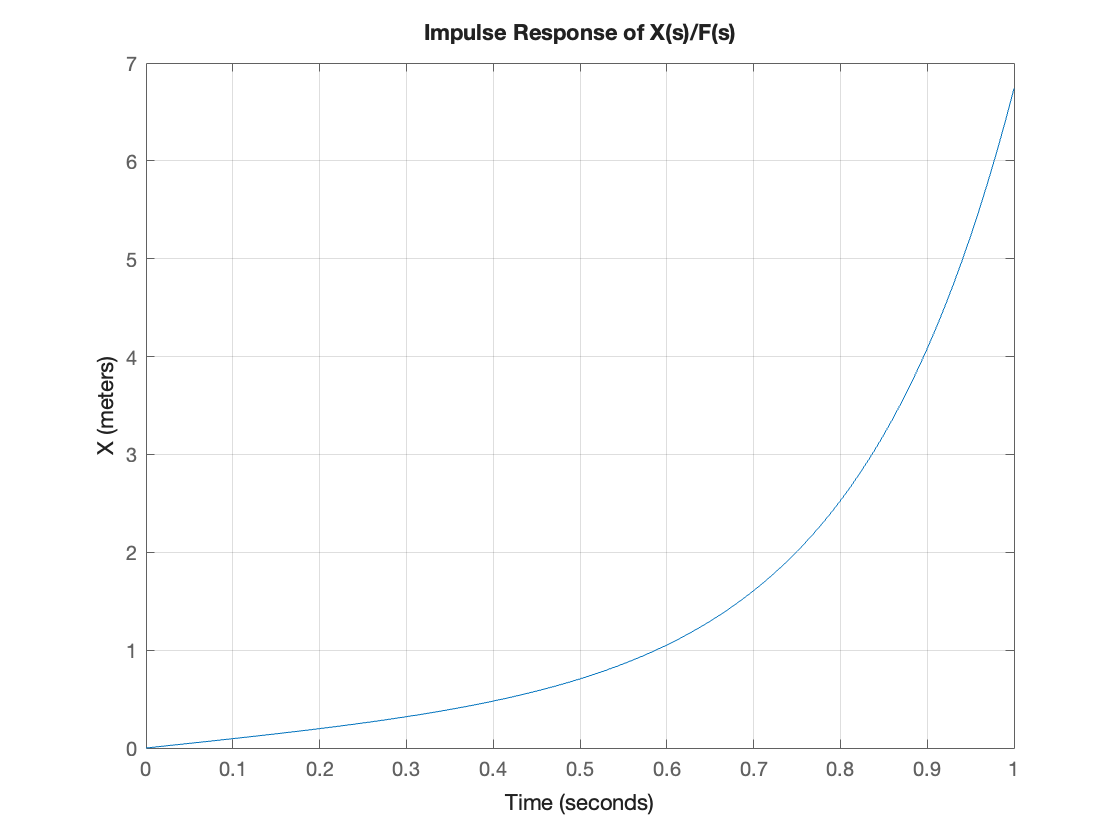
\includegraphics[width=0.5\textwidth]{p1dc.png}
    \caption{Impulse Response of X(s)/F(s)}
\end{figure}




\newpage
\subsection*{(e) (10pt)}

Now, consider the following feedback system with \( H(s) \) given by
\[
H(s) = K_p + \frac{K_i}{s} + K_d s.
\]
Plot three different impulse responses (10 seconds) for the closed-loop system with the following three different gains. Note that \( G(s) = \frac{\Theta(s)}{F(s)} \) from (b).
\[
K_p = 50, \quad K_i = 0, \quad K_d = 1
\]
\[
K_p = 50, \quad K_i = 1, \quad K_d = 0
\]
\[
K_p = 50, \quad K_i = 1, \quad K_d = 1
\]


\begin{lstlisting}
clc
clear
close all

% MATLAB code to plot the impulse responses for different PID gains

% Given constants
M = 1;          % Mass M in kg
m = 0.5;        % Mass m in kg
b = 0.2;        % Damping coefficient in N*m^{-1}*s
l = 0.4;        % Length l in meters
J = 0.01;       % Moment of inertia J in kg*m^2
g = 9.8;        % Acceleration due to gravity in m/s^2

% Calculations
ml = m * l;
ml2 = m * l^2;
ml_squared = (m * l)^2;
J_plus_ml2 = J + ml2;
M_plus_m = M + m;

% Denominator coefficients for Theta(s)/F(s)
a4 = (J_plus_ml2) * M_plus_m - ml_squared;  % s^4
a3 = (J_plus_ml2) * b;                      % s^3
a2 = -m * g * l * M_plus_m;                 % s^2
a1 = -m * g * l * b;                        % s^1
a0 = 0;                                     % s^0

den_theta = [a4, a3, a2, a1, a0];

% Numerator coefficients for Theta(s)/F(s)
num_theta = [0, 0, ml, 0, 0];

% Create the transfer function for Theta(s)/F(s)
G_s = tf(num_theta, den_theta);

% Time vector for impulse response (10 seconds)
t = linspace(0, 10, 1000);

% Define the three sets of PID gains
gains = [
    50, 0, 1;  % Kp = 50, Ki = 0, Kd = 1
    50, 1, 0;  % Kp = 50, Ki = 1, Kd = 0
    50, 1, 1   % Kp = 50, Ki = 1, Kd = 1
];

% Loop over each set of gains
for i = 1:size(gains, 1)
    K_p = gains(i, 1);
    K_i = gains(i, 2);
    K_d = gains(i, 3);
    
    % Define the PID controller H(s)
    num_H = [K_d, K_p, K_i];  % Numerator coefficients
    den_H = [1, 0];           % Denominator coefficients (s)
    H_s = tf(num_H, den_H);
    
    % Open-loop transfer function: G(s) * H(s)
    OpenLoop = series(H_s, G_s);
    
    % Closed-loop transfer function with unity feedback
    ClosedLoop = feedback(OpenLoop, 1);
    
    % Plot the impulse response
    figure;
    impulse(ClosedLoop, t);
    title(['Impulse Response for K_p = ', num2str(K_p), ...
           ', K_i = ', num2str(K_i), ', K_d = ', num2str(K_d)]);
    xlabel('Time (seconds)');
    ylabel('\Theta (radians)');
    grid on;
    
    % Save the figure
    saveas(gcf, ['p1e', num2str(i), '.png']);
end
\end{lstlisting}


\begin{figure}[h!]
    \centering
    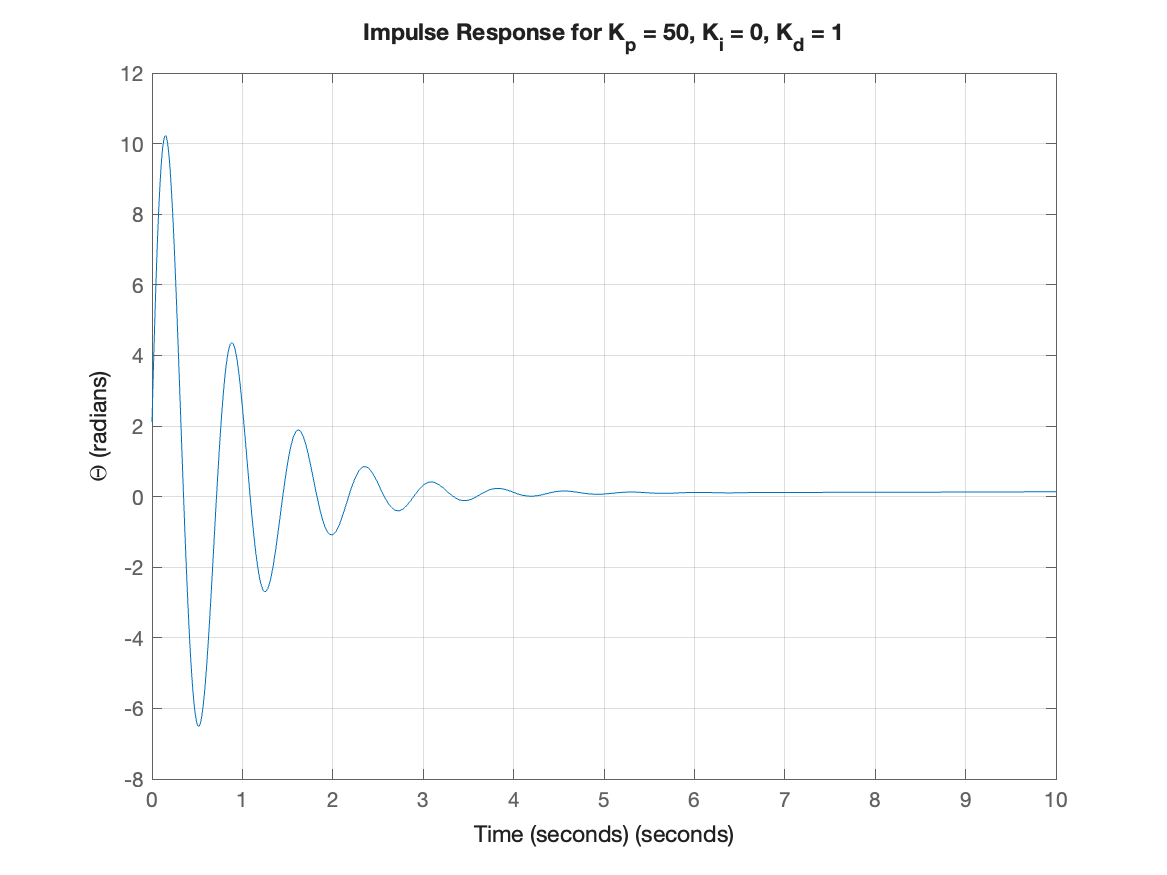
\includegraphics[width=0.45\textwidth]{p1e1.png}
    \caption{Impulse Response for $K_p = 50$, $K_i = 0$, $K_d = 1$}
\end{figure}
\newpage
\begin{figure}[h!]
    \centering
    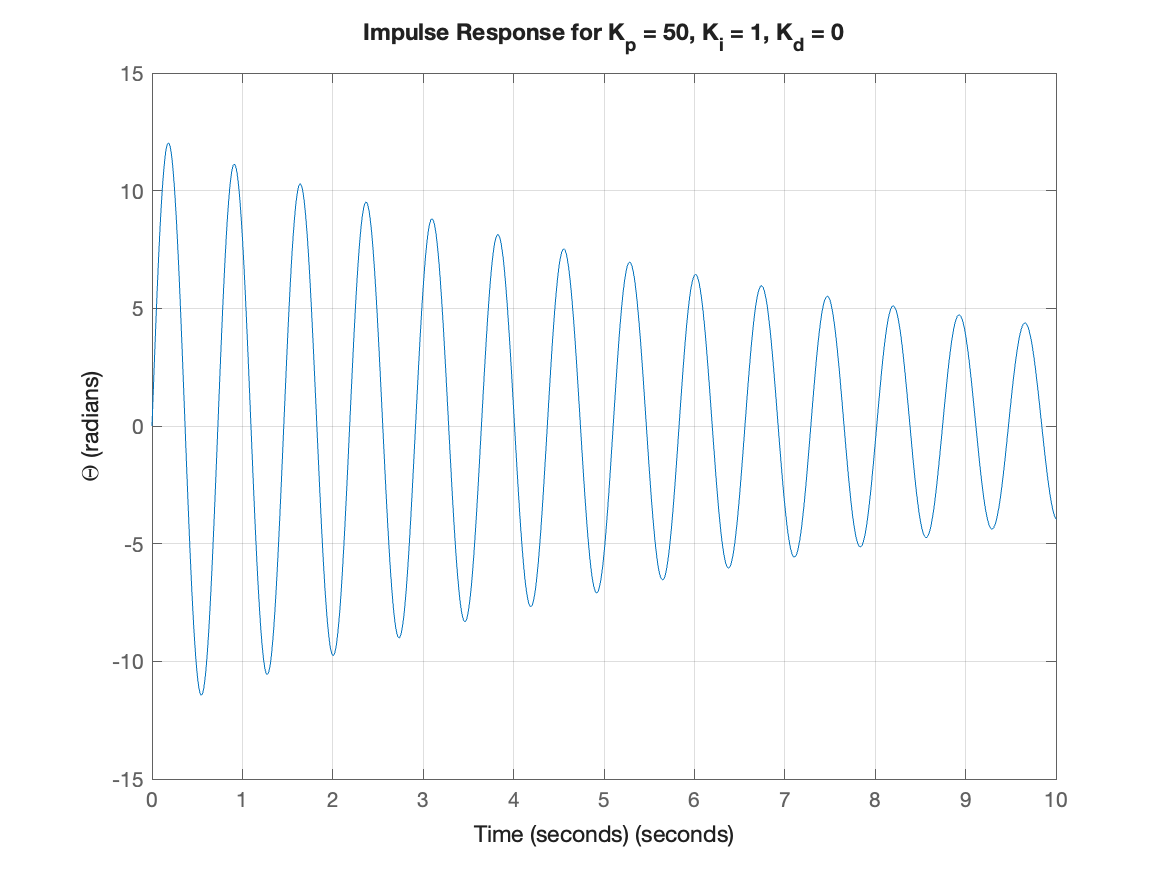
\includegraphics[width=0.45\textwidth]{p1e2.png}
    \caption{Impulse Response for $K_p = 50$, $K_i = 1$, $K_d = 0$}
\end{figure}

\begin{figure}[h!]
    \centering
    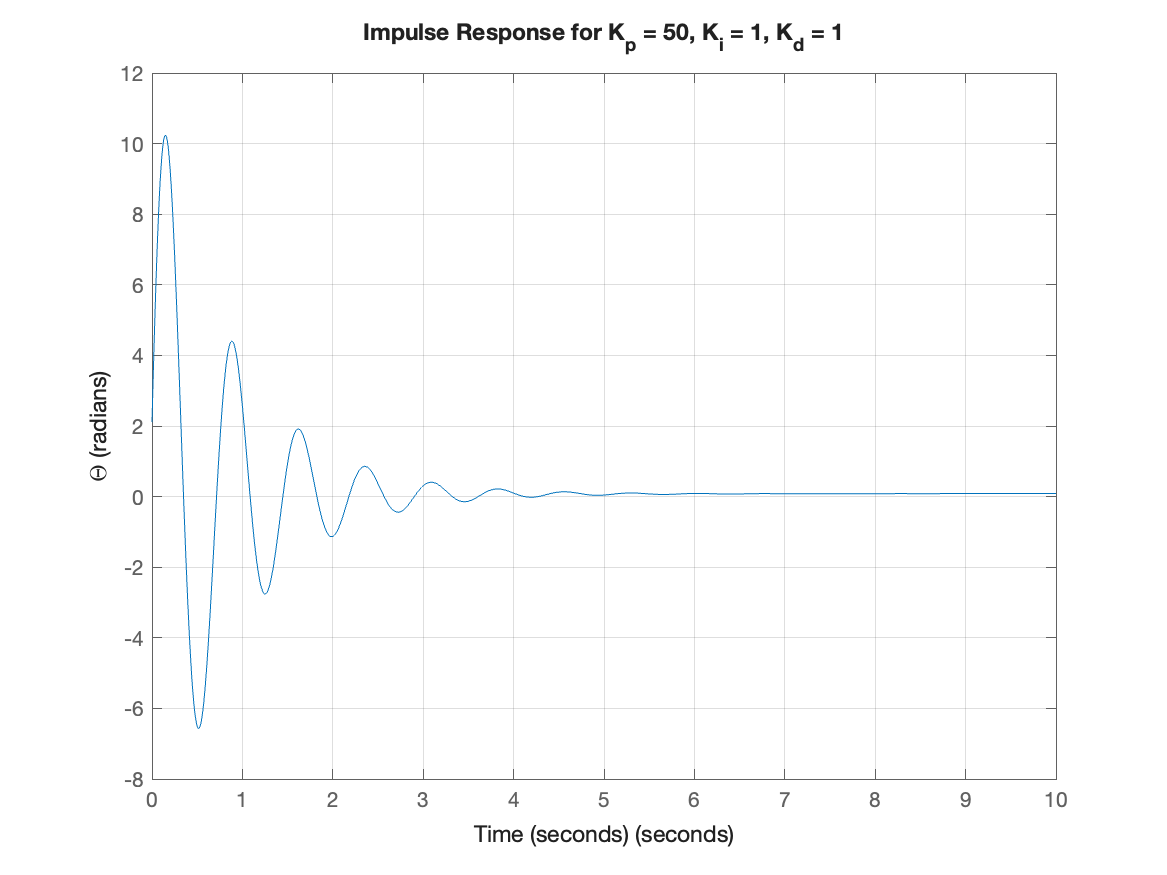
\includegraphics[width=0.45\textwidth]{p1e3.png}
    \caption{Impulse Response for $K_p = 50$, $K_i = 1$, $K_d = 1$}
\end{figure}

\newpage
\subsection*{(f) (10pt)}

Compare the results from (e). What are the differences among PD, PI, and PID controllers? (Hint: Zoom in for the steady state.)

The impulse response results for PD, PI, and PID controllers reveal distinct differences in their behavior, particularly in terms of oscillation and steady-state performance. By zooming in on the steady-state region, we observe the following:

\begin{itemize}
    \item \textbf{PD Controller} ($K_p = 50$, $K_i = 0$, $K_d = 1$): The PD controller has a small steady-state error and oscillates minimally in the final stages. This type of controller effectively reduces the overshoot and improves response time but cannot eliminate steady-state error completely because it lacks an integral term.
    
    \item \textbf{PI Controller} ($K_p = 50$, $K_i = 1$, $K_d = 0$): The PI controller exhibits significant oscillations compared to the PD controller. However, over time, the integral action works to eliminate the steady-state error entirely, which is a primary benefit of using a PI controller. The lack of derivative control means this system has less damping, resulting in sustained oscillations before settling.
    
    \item \textbf{PID Controller} ($K_p = 50$, $K_i = 1$, $K_d = 1$): The PID controller combines the benefits of both the PI and PD controllers. As observed in the zoomed-in steady-state, it achieves both minimal oscillations and reduction of the steady-state error( a Ki of 2 almost eliminates $e_{ss}$). The derivative term helps in reducing overshoot and oscillations, while the integral term ensures no steady-state error.
\end{itemize}

In conclusion, the PID controller provides the best overall performance by reducing oscillations (due to the derivative term) and reducing the steady-state error (due to the integral term), offering a balance of stability and accuracy.

\newpage
\subsection*{(g) (20pt)}

Consider the following feedback system with \( H(s) \) given by
\[
H(s) = 0.02s + 1 + \frac{0.02}{s}.
\]
Draw the root locus with MATLAB and find the closed-loop poles with \( K = 50 \).

Below is the MATLAB code used to plot the root locus of the open-loop transfer function \( L(s) = G(s)H(s) \) and determine the closed-loop poles for \( K = 50 \).

\begin{lstlisting}[language=Matlab, caption={MATLAB Code for Root Locus and Closed-Loop Poles}]
% MATLAB code to plot the root locus and find closed-loop poles at K = 50

% Clear workspace and command window
clear;
close all;
clc;

% Given constants
M = 1;          % Mass M in kg
m = 0.5;        % Mass m in kg
b = 0.2;        % Damping coefficient in N*m^{-1}*s
l = 0.4;        % Length l in meters
J = 0.01;       % Moment of inertia J in kg*m^2
g = 9.8;        % Acceleration due to gravity in m/s^2

% Intermediate calculations for G(s)
ml = m * l;
ml2 = m * l^2;
ml_squared = (m * l)^2;
J_plus_ml2 = J + ml2;
M_plus_m = M + m;

% Denominator coefficients for G(s)
a4 = (J_plus_ml2) * M_plus_m - ml_squared;  % s^4 coefficient
a3 = (J_plus_ml2) * b;                      % s^3 coefficient
a2 = -m * g * l * M_plus_m;                 % s^2 coefficient
a1 = -m * g * l * b;                        % s^1 coefficient
a0 = 0;                                      % s^0 coefficient

den_G = [a4, a3, a2, a1, a0];  % Denominator of G(s)

% Numerator coefficients for G(s)
num_G = [0, 0, ml, 0, 0];  % Numerator of G(s)

% Create the transfer function G(s)
G_s = tf(num_G, den_G);

% Define H(s)
% H(s) = 0.02s + 1 + 0.02/s = (0.02s^2 + s + 0.02)/s
num_H = [0.02, 1, 0.02];  % Numerator coefficients of H(s)
den_H = [1, 0];            % Denominator coefficients of H(s) (s)

H_s = tf(num_H, den_H);

% Open-loop transfer function L(s) = K * G(s) * H(s)
% Since K is variable, we define L(s) without K
L_without_K = series(G_s, H_s);  % Equivalent to G(s) * H(s)

% Plot the Root Locus
figure;
rlocus(L_without_K);
title('Root Locus of Open-Loop Transfer Function L(s) = G(s)H(s)');
xlabel('Real Axis');
ylabel('Imaginary Axis');
grid on;

% Define Gain K
K = 50;

% Modify L(s) to include gain K
L_with_K = K * L_without_K;

% Closed-loop transfer function T(s) = L(s) / (1 + L(s))
T_s = feedback(L_with_K, 1);

% Display the Closed-Loop Transfer Function
disp('Closed-loop Transfer Function T(s):');
disp(T_s);

% Find Closed-Loop Poles
closed_loop_poles = pole(T_s);
disp('Closed-loop poles at K = 50:');
disp(closed_loop_poles);

% Plot the Pole-Zero Map of Closed-Loop System
figure;
pzmap(T_s);
title(['Pole-Zero Map of Closed-Loop Transfer Function T(s) at K = ', num2str(K)]);
xlabel('Real Axis');
ylabel('Imaginary Axis');
grid on;

% Optional: Highlight Closed-Loop Poles on Root Locus
figure;
rlocus(L_without_K);
hold on;
sgrid;
% Mark the closed-loop poles
plot(real(closed_loop_poles), imag(closed_loop_poles), 'rx', 'MarkerSize', 12, 'LineWidth', 2);
title(['Root Locus with Closed-Loop Poles at K = ', num2str(K)]);
xlabel('Real Axis');
ylabel('Imaginary Axis');
grid on;
hold off;
\end{lstlisting}

\subsection*{Closed-Loop Pole Locations for \( K = 50 \)}
For a gain value of \( K = 50 \), the closed-loop poles of the system are located at the following positions in the complex plane:

\begin{align*}
s_1 &= 0.0000 + 0.0000i \quad (\text{Multiplicity}) \\
s_2 &= -1.1610 + 8.5458i \\
s_3 &= -1.1610 - 8.5458i \\
s_4 &= 0.0272 + 0.0000i \\
\end{align*}
\begin{itemize}
    \item \(\mathbf{s_1}\) Pole is located at the origin (\(s = 0\)), indicating an integrative component in the system.
    
    \item \(\mathbf{s_2 \text{ and } s_3:}\) These complex conjugate poles are located in the left-half of the complex plane, suggesting stable oscillatory behavior with a natural frequency and damping ratio determined by their real and imaginary parts.
    
    \item \(\mathbf{s_4:}\) This pole is located slightly to the right of the imaginary axis (\(s = 0.0272\)), indicating instability. A pole in the right-half plane means that the system will exhibit unbounded growth in response to disturbances or inputs.
\end{itemize}
\newpage
\begin{figure}[h]
    \centering
    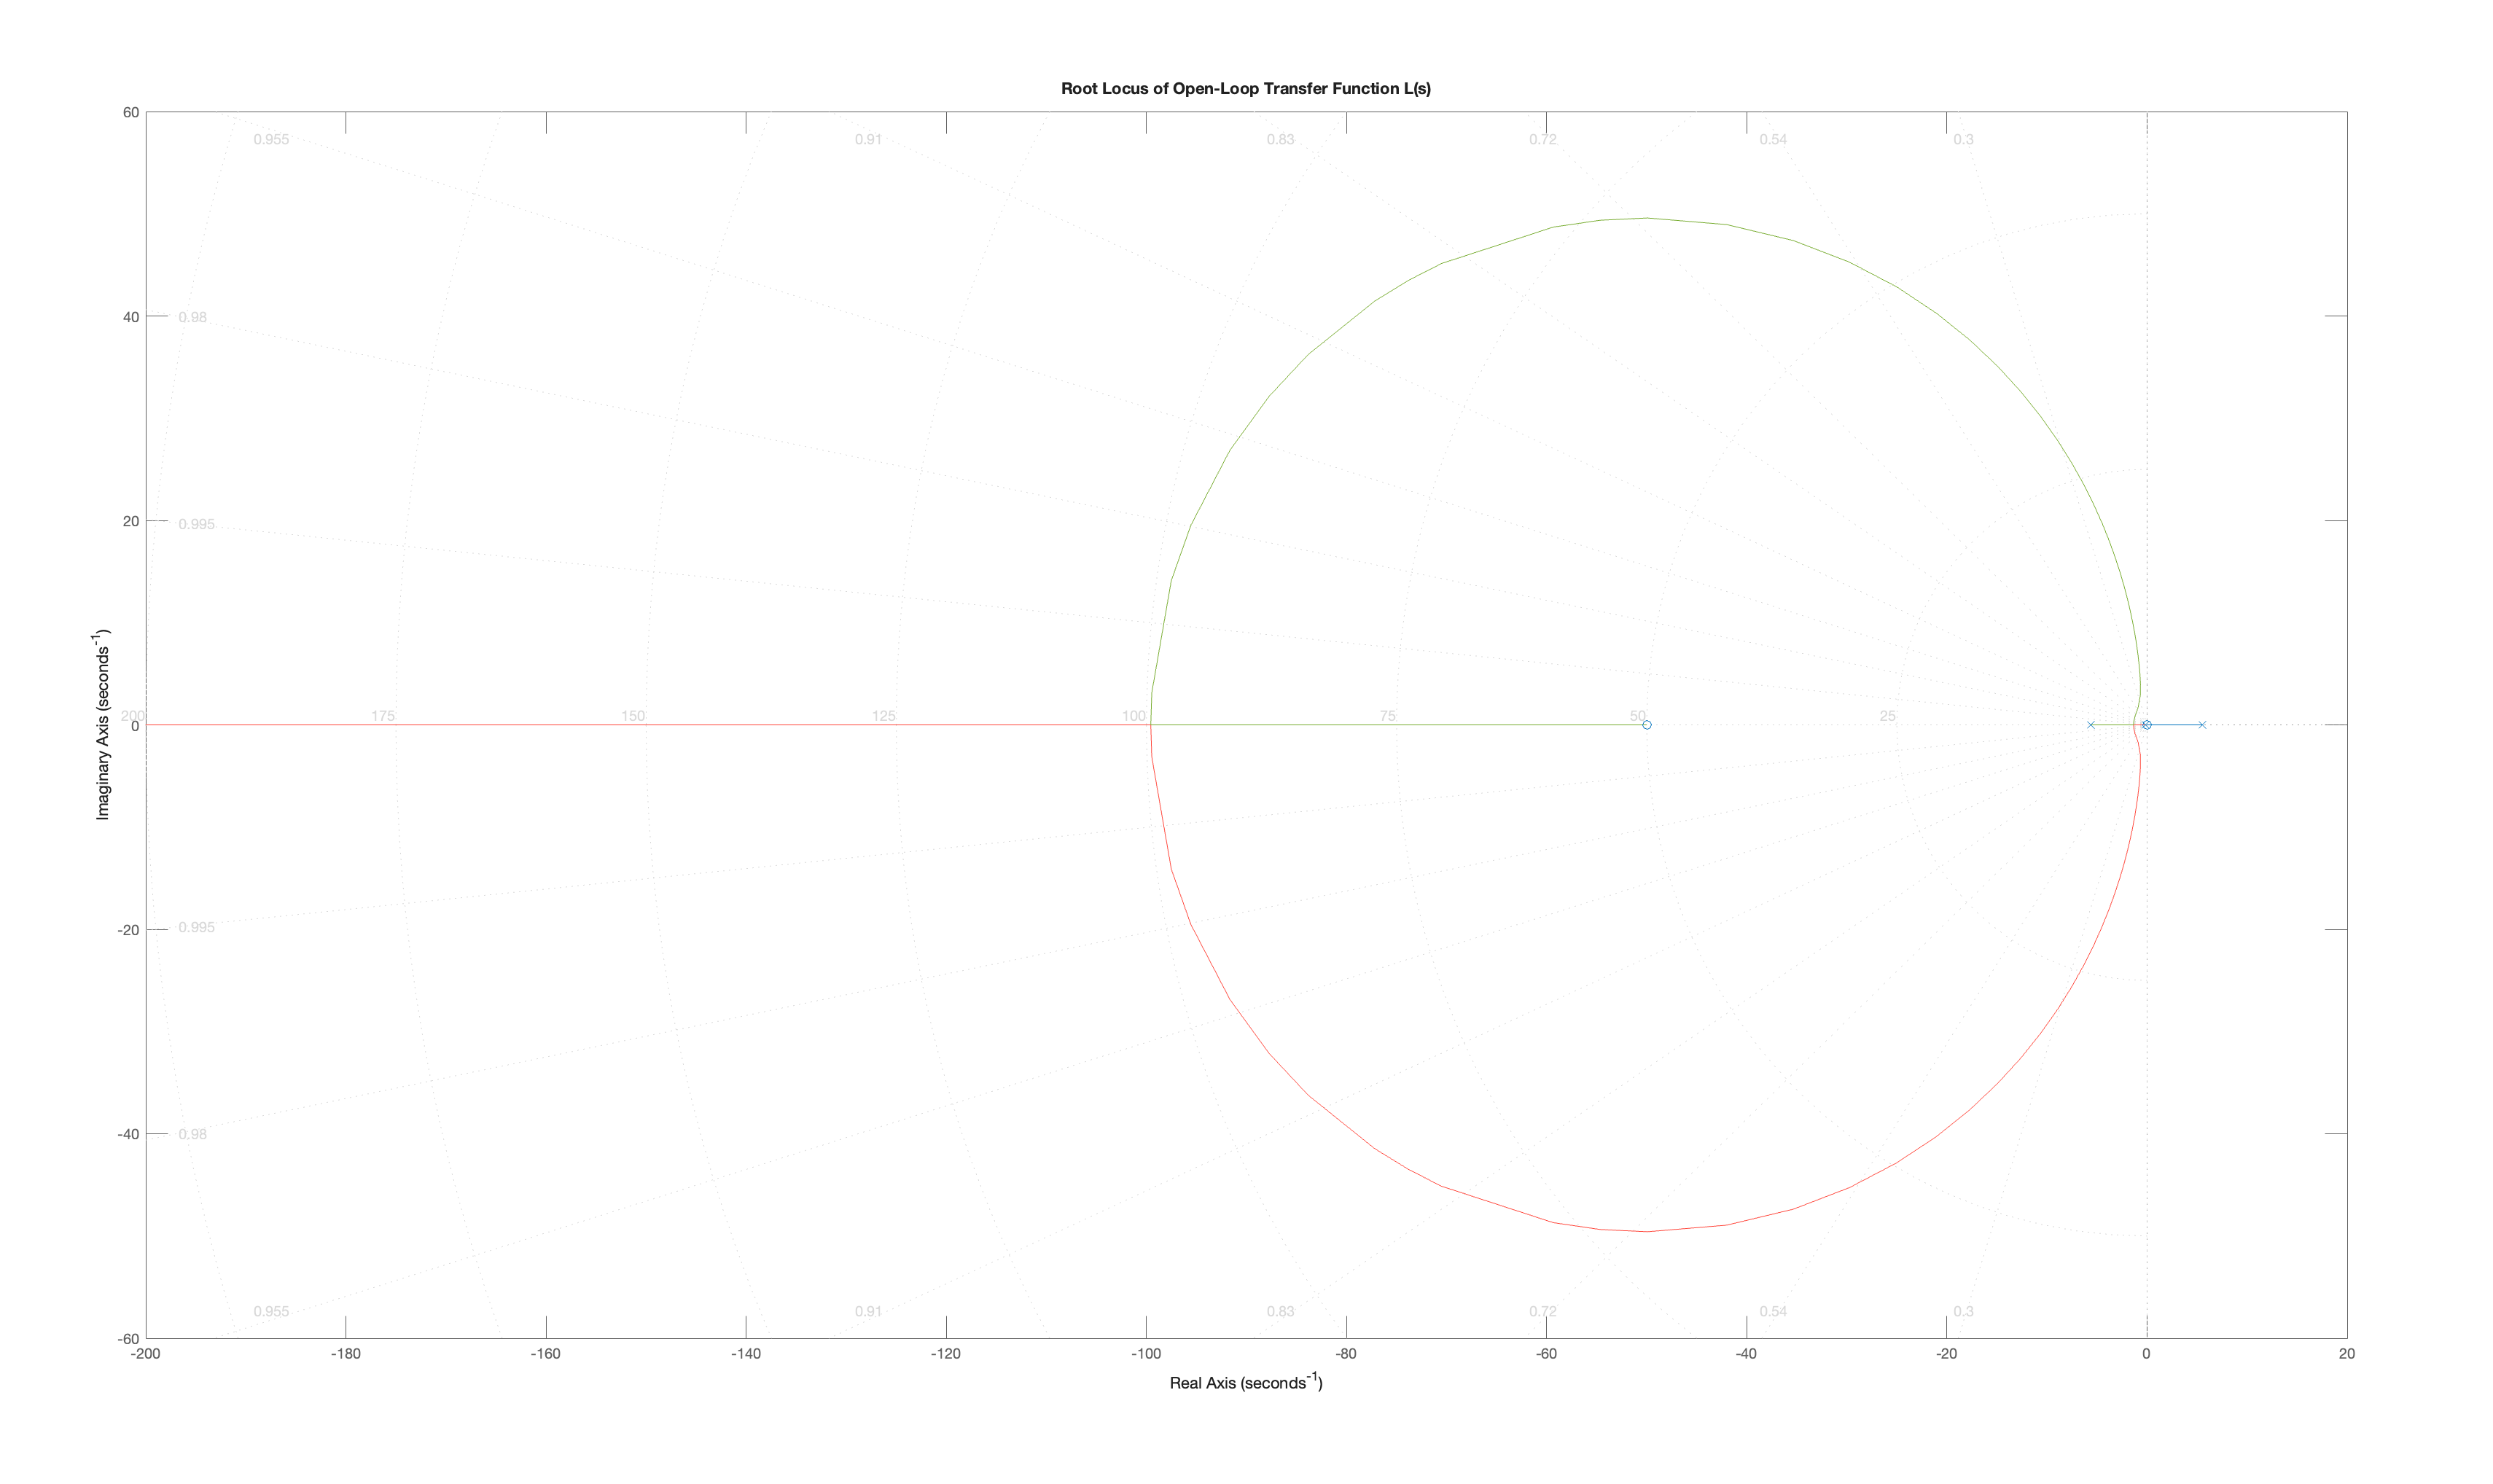
\includegraphics[width=0.8\textwidth]{root_locus.png} % Replace with your image file name
    \caption{Root Locus of the Open-Loop Transfer Function \( L(s) = G(s)H(s) \)}
    \label{fig:root_locus}
\end{figure}
\newpage
\section*{Problem 2 (20pt)}

Consider the following 2nd order system:
\[
\frac{X(s)}{F(s)} = G(s) = \frac{\omega_n^2}{s^2 + 2\zeta \omega_n s + \omega_n^2}.
\]
The step response has the following performance indicators: 
\[
t_s = 4 \, \text{s}, \quad t_p = 0.81 \, \text{s}, \quad x_p = 1.44.
\]
Find \( \zeta \) and \( \omega_n \). (Round \( \zeta \) to the nearest hundredth and \( \omega_n \) to the nearest integer.)
\newline\newline
For a standard second-order system, the key performance indicators are related to \( \zeta \) and \( \omega_n \) as follows:

\noindent
1. \textbf{Peak Time (\( t_p \))}:
   \[
   t_p = \frac{\pi}{\omega_n \sqrt{1 - \zeta^2}}
   \]
\noindent
2. \textbf{Settling Time (\( t_s \))} (using the 2\% criterion):
   \[
   t_s \approx \frac{4}{\zeta \omega_n}
   \]
\noindent
3. \textbf{Percent Overshoot (\( \%PO \))}:
   \[
   \%PO = e^{\left(-\frac{\pi \zeta}{\sqrt{1 - \zeta^2}}\right)} \times 100\%
   \]
   Given \( x_p = 1.44 \), the percent overshoot is:
   \[
   \%PO = (1.44 - 1) \times 100\% = 44\%
   \]

\noindent
From the settling time:
\[
t_s = \frac{4}{\zeta \omega_n} \implies \zeta \omega_n = \frac{4}{t_s} = \frac{4}{4} = 1
\]
\[
\omega_n = \frac{1}{\zeta}
\]
\noindent
From the peak time:
\[
t_p = \frac{\pi}{\omega_n \sqrt{1 - \zeta^2}} \implies t_p = \frac{\pi \zeta}{\sqrt{1 - \zeta^2}} = 0.81
\]
\[
\frac{\pi \zeta}{\sqrt{1 - \zeta^2}} = 0.81
\]

\noindent
Square both sides to eliminate the square root:
\[
\left(\frac{\pi \zeta}{\sqrt{1 - \zeta^2}}\right)^2 = 0.81^2
\]
\[
\frac{\pi^2 \zeta^2}{1 - \zeta^2} = 0.6561
\]
\[
\pi^2 \zeta^2 = 0.6561 (1 - \zeta^2)
\]
\[
\zeta^2 (\pi^2 + 0.6561) = 0.6561
\]
\[
\zeta^2 = \frac{0.6561}{\pi^2 + 0.6561} \approx \frac{0.6561}{10.5257} \approx 0.06238
\]
\[
\zeta \approx \sqrt{0.06238} \approx 0.25
\]

\noindent
Using \( \zeta \omega_n = 1 \):
\[
\omega_n = \frac{1}{\zeta} = \frac{1}{0.25} = 4 \, \text{rad/s}
\]

\[
\boxed{\,\zeta = 0.25 \quad \text{and} \quad \omega_n = 4\,}
\]



\newpage
\section*{Bonus Problem (20pt)}

\subsection*{(a) (10pt) Routh Stability Criteria}

\noindent
What are the two criteria for the Routh stability condition?

\subsubsection*{Answer:}
The Routh-Hurwitz stability criterion is used to assess the stability of a linear time-invariant (LTI) system by analyzing the characteristic equation. The two primary criteria are:

\begin{enumerate}
    \item \textbf{All Coefficients Must Be Positive:} For a system to be stable, all coefficients of the characteristic equation should be positive. Any negative coefficient indicates the presence of poles with positive real parts, implying instability.
    
    \item \textbf{No Sign Changes in the First Column of the Routh Table:} Once the Routh table is constructed, the first column is checked for sign changes. The number of sign changes corresponds to the number of poles with positive real parts. For stability, no sign changes should occur, ensuring that all poles are in the left half-plane.
\end{enumerate}

\subsection*{(b) (10pt) Controller Selection}

\noindent
The step response of your open-loop system is given as follows. What controllers should you use to eliminate the steady-state error? Select all that apply and explain why.

\begin{enumerate}
    \item P
    \item PI
    \item PD
    \item PID
    \item None of the above
\end{enumerate}

\subsubsection*{Answer:}
To eliminate the steady-state error, the controllers with integral action are most effective, as the integral term accumulates the error and adjusts the control input accordingly. The following controllers are suitable:

\begin{enumerate}
    \item \textbf{PI (Proportional-Integral) Controller:} The integral component in the PI controller helps eliminate steady-state error by continuously adjusting the control input based on the accumulated error.
    
    \item \textbf{PID (Proportional-Integral-Derivative) Controller:} In addition to the integral action, the derivative component improves the transient response, while the proportional and integral components work together to eliminate steady-state error.
\end{enumerate}

\noindent
Thus, the appropriate controllers to select are:
\begin{itemize}
    \item \textbf{PI (2)}
    \item \textbf{PID (4)}
\end{itemize}

\noindent
Both PI and PID controllers introduce integral action, which is necessary to eliminate steady-state error. The PID controller additionally improves system stability through its derivative component.


\end{document}
